\documentclass{article}

\usepackage{fancyhdr}
\usepackage{extramarks}
\usepackage{amsmath,siunitx}
\usepackage{amsthm}
\usepackage{bm}
\usepackage{amssymb}
\usepackage{amsfonts}
\usepackage{multirow}
\usepackage{tikz}
\usepackage[plain]{algorithm}
\usepackage{algpseudocode}
\usepackage{changepage}
\usepackage{color}


\usetikzlibrary{automata,positioning}


%
% Basic Document Settings
%

\topmargin=-0.45in
\evensidemargin=0in
\oddsidemargin=0in
\textwidth=6.5in
\textheight=9.0in
\headsep=0.25in

\linespread{1.1}

\pagestyle{fancy}
% \lhead{\hmwkTeam}
\chead{\hmwkClass: \hmwkTitle}
\rhead{\firstxmark}
\lfoot{\lastxmark}
\cfoot{\thepage}

\renewcommand\headrulewidth{0.4pt}
\renewcommand\footrulewidth{0.4pt}

\setlength\parindent{0pt}

\newcommand{\setsep}{,    \ }

%
% Create Problem Sections
%

\newcommand{\enterProblemHeader}[1]{
    \nobreak\extramarks{}{Problem \hmwkNumber.\arabic{#1} continued on next page\ldots}\nobreak{}
    \nobreak\extramarks{Problem \hmwkNumber.\arabic{#1} (continued)}{Problem \hmwkNumber.\arabic{#1} continued on next page\ldots}\nobreak{}
}

\newcommand{\exitProblemHeader}[1]{
    \nobreak\extramarks{Problem \hmwkNumber.\arabic{#1} (continued)}{Problem \hmwkNumber.\arabic{#1} continued on next page\ldots}\nobreak{}
    \stepcounter{#1}
    \nobreak\extramarks{Problem \hmwkNumber.\arabic{#1}}{}\nobreak{}
}

\setcounter{secnumdepth}{0}
\newcounter{partCounter}
\newcounter{homeworkProblemCounter}
\setcounter{homeworkProblemCounter}{1}
\nobreak\extramarks{Problem \arabic{homeworkProblemCounter}}{}\nobreak{}

%
% Homework Problem Environment
%
% This environment takes an optional argument. When given, it will adjust the
% problem counter. This is useful for when the problems given for your
% assignment aren't sequential. See the last 3 problems of this template for an
% example.
%
\newenvironment{homeworkProblem}[2][-2]{
    \ifnum#1>0
        \setcounter{homeworkProblemCounter}{#1}
    \fi
    \section{Problem \hmwkNumber.\arabic{homeworkProblemCounter} #2}
    \setcounter{partCounter}{1}
    \enterProblemHeader{homeworkProblemCounter}
}{
    \exitProblemHeader{homeworkProblemCounter}
}

%
% Homework Details
%   - Title
%   - Due date
%   - Class
%   - Section/Time
%   - Instructor
%   - Author
%
\newcommand{\hmwkNumber}{E22}
\newcommand{\hmwkTitle}{Exam 2022}
\newcommand{\hmwkClass}{NNTI}
% \newcommand{\hmwkTeam}{Team \#25}
\newcommand{\hmwkAuthorName}{Jackie, Camilo, Kai, Dhimitrios, Hevra}

%
% Title Page
%

\title{
    % \vspace{2in}
    \textmd{\textbf{\hmwkClass:\ \hmwkTitle}}\\
}

\author{\hmwkAuthorName}
\date \today

\renewcommand{\part}[1]{\textbf{\large Part \Alph{partCounter}}\stepcounter{partCounter}\\}

%
% Various Helper Commands
%

% Useful for algorithms
\newcommand{\alg}[1]{\textsc{\bfseries \footnotesize #1}}

% For derivatives
\newcommand{\deriv}[1]{\frac{\mathrm{d}}{\mathrm{d}x} (#1)}

% For partial derivatives
\newcommand{\pderiv}[2]{\frac{\partial}{\partial #1} (#2)}

% Integral dx
\newcommand{\dx}{\mathrm{d}x}

% Alias for the Solution section header
\newcommand{\solution}{\textbf{\large Solution}}

% Probability commands: Expectation, Variance, Covariance, Bias
\newcommand{\E}{\mathrm{E}}
\newcommand{\Var}{\mathrm{Var}}
\newcommand{\Cov}{\mathrm{Cov}}
\newcommand{\Bias}{\mathrm{Bias}}

\newenvironment{homeworkSubsection}{\begin{adjustwidth}{2.5em}{0pt}}{\end{adjustwidth}}
\newcommand{\red}[1]{\textcolor{red}{#1}}
\begin{document}

\maketitle

\begin{homeworkProblem}{Short questions}
    \subsection*{(a)}
    \begin{homeworkSubsection}
        (i) is not a good candidate because the derivative is 0 that will make gradient vanish.
        (ii) is not a good candidate because the network is limited to learn only quadratic functions.
        (iii) Uhh.. what is the normal distribution formular doing here?
    \end{homeworkSubsection}
    \subsection*{(b)}
    \begin{homeworkSubsection}
        (ii) is correct because a deep network will face a problem called covariance shift
        , that is the variance of the intermediate layer output may change after the weights from the previous layer being updated.
        Batch norm make sure that the variance of such layer so we can introduce a higher learning rate to the network
        thus speeds up the convergence.
    \end{homeworkSubsection}
    \subsection*{(c)}
    \begin{homeworkSubsection}
        Batch Size = 1? The batch norm video from Andrew Ng says batch norm is applied to the intermediate layer output. Confused.
    \end{homeworkSubsection}
    \subsection*{(d)}
    \begin{homeworkSubsection}
        (i) Yes because the kernel depth has to match the input volumn depth

        (ii) Yes, usually one bias per kernel/filter.

        (iii) No because it only affects output dimension.

        (iv) No because it only affects output dimension.

    \end{homeworkSubsection}
    \subsection*{(e)}
    \begin{homeworkSubsection}
        Datasets that are not linearly separable are difficult for a linear classifier to correctly
        classify.
    \end{homeworkSubsection}
    \subsection*{(f)}
    \begin{homeworkSubsection}
        Because it is computationally expensive.
    \end{homeworkSubsection}
    \subsection*{(g)}
    \begin{homeworkSubsection}
        Max pooling can make the kernels pick up feature even if it is rotated.
    \end{homeworkSubsection}
    \subsection*{(h)}
    \begin{homeworkSubsection}
        It is not a good idea because sigmoid's exponential term may be overflow.
    \end{homeworkSubsection}
    \subsection*{\red{(i)}}
    \subsection*{\red{(j)}}
\end{homeworkProblem}
\begin{homeworkProblem}{Principal Component Analysis (PCA)}
    \subsection*{(a)}
    \begin{homeworkSubsection}
        The first assumption is that the dataset are centered at 0
        i.e. the mean is substracted from each data point
        because PCA trys to project the points on the the pca hyperplane (or line)
        so that the variance of the original dataset does not change much
        and the new axes are go through the original.

        The second one is that the dataset is normalized
        because different variables (axes) have different scales.
        Their covariances are not comparable if the data are not under the same scale.
    \end{homeworkSubsection}
    \subsection*{(b)}
    \begin{homeworkSubsection}
        The objective function is given by:
        \[
            \underset{D}{\mathrm{argmin}}\underset{i}{\sum}||x^{(i)}-DD^\top x^{(i)}||
        \]
        where matrix $D \in \mathbb{R}^{m\times l}$ and vectors $x^{(i)} \in \mathbb{R}^{m}$.
        We are looking for a matrix $D$ that tranforms $x^{(i)}$ into a lower dimention($l$) space
        and minimizes the reconstruction error.
    \end{homeworkSubsection}
    \subsection*{(c)}
    \subsection*{(d)}
    \begin{homeworkSubsection}
        From A3.2b we know that the objective function can also be written as
        $\underset{D}{\mathrm{argmin}}||X-XDD^\top||_F^2$ and later derived as
        $\underset{D}{\mathrm{argmax}}\sum_{i=1}^{m}D_{.i}^\top X^\top XD_{.i}$
        where $D_{.i}$ is a column of $D$.
        We simplify the problem by treating $D_{.i}$ as a vector $d$ with constraint $d^\top d = 1$:
        \begin{align*}
            \underset{d}{\mathrm{argmax}}d^\top X^\top Xd
            &= \underset{d}{\mathrm{argmax}}(Xd)^2\\
            &= \underset{d}{\mathrm{argmax}}\sum_{i=1}^{n}(d^\top x^{(i)})^2\\
            &= \underset{d}{\mathrm{argmax}}\frac{1}{n}\sum_{i=1}^{n}(d^\top x^{(i)} - 0)^2
        \end{align*}
        One can observe that the formular $\frac{1}{n}\sum_{i=1}^{n}(d^\top x^{(i)} - 0)^2$ is 
        calculating the variance of the points projected onto direction $d$ (note that the mean is 0 from assumption).
    \end{homeworkSubsection}
\end{homeworkProblem}
\begin{homeworkProblem}{Machine Learning Basics}
    \subsection*{(a)}
    \begin{homeworkSubsection}
        We have the loss function $J(w) = \frac{1}{n}||Xw-y||^2_2 + \lambda w^\top w$.
        We can find the $w$ minimizes $J(W)$ by setting the gradient $\nabla_wJ(w) = 0$.
        \begin{align*}
            \nabla_wJ(w) &= 0\\
            \frac{2}{n}X^\top(Xw-y) + 2\lambda w &= 0\\
            X^\top Xw-X^\top y + n\lambda w &= 0\\
            (X^\top X + n\lambda I)w-X^\top y &= 0\\
            (X^\top X + n\lambda I)w &= X^\top y \\
            w  &=(X^\top X + n\lambda I)^{-1}X^\top y\\
        \end{align*}
    \end{homeworkSubsection}
    \subsection*{(b)}
    \begin{homeworkSubsection}
        The equation is the same as $J(w) = \frac{1}{2}||Xw-y||^2_2 + \alpha ||w||_1  + \frac{\lambda}{2}w^Tw$.
        One can observe that there is an L1 norm in the equation.
        The derivative of L1 norm cannot be expressed as a closed form because it depends on the sign of each element in vector $w$.
    \end{homeworkSubsection}
    \subsection*{(c)}
    \begin{homeworkSubsection}
        Now we have the $J(w) = \frac{1}{n}||Xw-y||^2_2 + \lambda w^\top T w$.
        Similarly we solve $\nabla_wJ(w) = 0$.
        \begin{align*}
            \frac{2}{n}X^\top(Xw-y) + \lambda (T + T^\top)w &= 0\\
            X^\top(Xw-y) + \frac{n\lambda}{2} (2T)w &= 0\\
            X^\top Xw- X^\top y + n\lambda Tw &= 0\\
            (X^\top X + n\lambda T)w &= X^\top y\\
            w &= (X^\top X + n\lambda T)^{-1}X^\top y\\
        \end{align*}
    \end{homeworkSubsection}
    \subsection*{(d)}
    \begin{homeworkSubsection}
        We can rewrite $w^\top w$ as $w^\top (ww^\top)^{\gamma-1} w$.
        Since $(ww^\top)^{\gamma-1}$ is symmetric matrix we can reuse the result from (c) and get
        \[
            w = (X^\top X + n\lambda (ww^\top)^{\gamma-1})^{-1}X^\top y\\
        \]
    \end{homeworkSubsection}
\end{homeworkProblem}
\begin{homeworkProblem}{Feed-Forward Neural Networks}
    \subsection*{(a)}
    \begin{homeworkSubsection}
        A deep nn can be computationally effecient as it can learn the same function with fewer parameters \red{Why?}
    \end{homeworkSubsection}
    \subsection*{(b)}
    \begin{homeworkSubsection}
        A saddle point is when the gradient is 0 (derivatives are 0 in both x and y direction)
        but the second derivatives in x and y direction are of different sign.
        As the gradient is 0, it may stop the gradient descent process even though it is not at a minimal.
    \end{homeworkSubsection}
    \subsection*{\red{(c)}}
    \subsection*{(d)}
    \begin{homeworkSubsection}
        MSE (Mean square error) measures the euclidean distance between the true value and the predicted one.
        It can be used for regression task.
        \red{Cross Entropy} can be used for classification task.
    \end{homeworkSubsection}
    \subsection*{(e)}
    \begin{homeworkSubsection}
        Quoted from Assignment 5.2:\\
        \textit{Consider a Neural Network with a single hidden layer consisting of M neurons and tanh
        activation function.For any neuron in the hidden layer, simultaneous change of sign of input
        and output weights from the neuron leads to no change in the output layer therefore producing
        an equivalent transformation.Similarly, for any pair of neurons interchange of input weights
        between the neurons and simultaneous interchange of output weights produces an equivalent
        transformation}
    \end{homeworkSubsection}
    \begin{homeworkSubsection}
    \end{homeworkSubsection}
\end{homeworkProblem}
\begin{homeworkProblem}{\red{Regularization}}
    
\end{homeworkProblem}
\begin{homeworkProblem}{Back propagation}
    \subsection*{(a)}
    \begin{homeworkSubsection}
        \[
            y = [\frac{27}{106}, \frac{1}{106}, \frac{2}{53}, \frac{27}{53}]
        \]
    \end{homeworkSubsection}
    \subsection*{(b)}
    \begin{homeworkSubsection}
        \begin{center}
            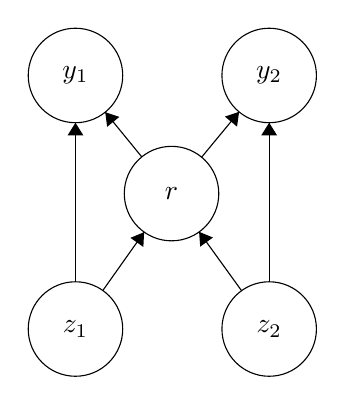
\begin{tikzpicture}[scale=0.2]
            \tikzstyle{every node}+=[inner sep=0pt]
            \draw [black] (27.5,-28.3) circle (3);
            \draw (27.5,-28.3) node {$z_1$};
            \draw [black] (39.8,-28.3) circle (3);
            \draw (39.8,-28.3) node {$z_2$};
            \draw [black] (33.6,-19.7) circle (3);
            \draw (33.6,-19.7) node {$r$};
            \draw [black] (27.5,-12.2) circle (3);
            \draw (27.5,-12.2) node {$y_1$};
            \draw [black] (39.8,-12.2) circle (3);
            \draw (39.8,-12.2) node {$y_2$};
            \draw [black] (38.05,-25.87) -- (35.35,-22.13);
            \fill [black] (35.35,-22.13) -- (35.42,-23.07) -- (36.23,-22.49);
            \draw [black] (29.24,-25.85) -- (31.86,-22.15);
            \fill [black] (31.86,-22.15) -- (30.99,-22.51) -- (31.81,-23.09);
            \draw [black] (27.5,-25.3) -- (27.5,-15.2);
            \fill [black] (27.5,-15.2) -- (27,-16) -- (28,-16);
            \draw [black] (39.8,-25.3) -- (39.8,-15.2);
            \fill [black] (39.8,-15.2) -- (39.3,-16) -- (40.3,-16);
            \draw [black] (35.51,-17.39) -- (37.89,-14.51);
            \fill [black] (37.89,-14.51) -- (36.99,-14.81) -- (37.76,-15.45);
            \draw [black] (31.71,-17.37) -- (29.39,-14.53);
            \fill [black] (29.39,-14.53) -- (29.51,-15.46) -- (30.29,-14.83);
            \end{tikzpicture}
            \end{center}
    \end{homeworkSubsection}
\end{homeworkProblem}


\end{document}